\documentclass[a4paper, 10pt]{article}
\usepackage[utf8]{inputenc} % Change according your file encoding
\usepackage{graphicx}
\usepackage{url}
\usepackage{amsmath}
\usepackage{amsthm}
\usepackage{algorithm}
\usepackage{multicol}
\usepackage[noend]{algpseudocode}
\usepackage{tikz}
\usetikzlibrary{shapes.geometric,positioning}
\usepackage[a4paper, left=2cm, right=2cm, top=2cm, bottom=2cm]{geometry}

\newtheorem{obs}{Observation}

%opening
\title{Seminar Report: [seminar ID] (e.g. Paxy)}
\author{\textbf{Name of team members}}
\date{\normalsize\today{}}

\begin{document}

% New definitions
\algnewcommand\algorithmicswitch{\textbf{switch}}
\algnewcommand\algorithmiccase{\textbf{case}}
\algnewcommand\algorithmicassert{\texttt{assert}}
\algnewcommand\Assert[1]{\State \algorithmicassert(#1)}%
% New "environments"
\algdef{SE}[SWITCH]{Switch}{EndSwitch}[1]{\algorithmicswitch\ #1\ \algorithmicdo}{\algorithmicend\ \algorithmicswitch}%
\algdef{SE}[CASE]{Case}{EndCase}[1]{\algorithmiccase\ #1}{\algorithmicend\ \algorithmiccase}%
\algtext*{EndSwitch}%
\algtext*{EndCase}%

%\maketitle
Carlos Segarra \hfill Thursday, September 26th

\vspace{15pt}

\textbf{\Large Discrete and Algorithmic Geometry: Problems 4 and 5}

\vspace{20pt}

\textbf{\textit{4. Propose an algorithm that, given a point $p$ external to a convex polygon $\mathcal{P}$, finds the point of $\mathcal{P}$ closest to $p$. What happens if instead of finding the closest point we look for the farthest? What if we restrict the search to the vertices of $\mathcal{P}$?}}

\vspace{3pt}

Let $\lbrace q_1, \dots, q_n\rbrace$ be the set of vertices of $\mathcal{P}$ in clock-wise order. And let $f$ be the function s.t. for all $q \in \mathcal{P}$, sends $p$ to $d(q, p)$. Before starting with the proof, let us make two observations:
\begin{obs}
    $f$ is an uni-modal application. Alternatively, its derivative is a linear funcion that has only one zero.
\end{obs}
\begin{obs} \label{obs-2}
    Let $q_{min}$ and $q_{min+1}$ be the closest and second to closest vertices from $\mathcal{P}$ to $p$. Then, the closest point in $\mathcal{P}$ to $p$ is either (i) $q_{min}$ or (ii) contained in the $q_{min}q_{min+1}$ segment.
\end{obs}

Note that the second observation applies symetrically to the farthest point in $\mathcal{P}$. 
Further, once we find the two closest points, checking wether we are in case (i) or case (ii) from Obs~\ref{obs-2} can be done in constant time testing if $p$ belongs to the triangle drawn by the line throguh $p$ parallel to $q_{min}q_{min+1}$ and the two lines through $p_{min}$ orthogonal to the segments incident to $p_{min}$.

\tikzset{
  my poly/.style={regular polygon, regular polygon sides=6,fill=gray!#1,minimum size=2cm, draw},
}

\begin{figure}[h!]
    \resizebox{\linewidth}{!}{
    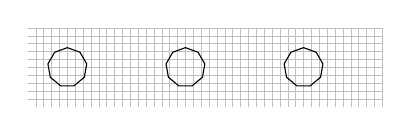
\begin{tikzpicture}[node distance=0pt, every node/.style={outer sep=0pt}]
        \draw [help lines,gray!50,step =0.1] (-0.5,-0.5) grid (4,0.5);
      %\node (1-C1) [my poly=10] {C1};
        \node (poly) [regular polygon, regular polygon sides=9, draw, minimum size = 0.5cm] at (0,0) {};
        \node (poly) [regular polygon, regular polygon sides=9, draw, minimum size = 0.5cm] at (1.5,0) {};
        \node (poly) [regular polygon, regular polygon sides=9, draw, minimum size = 0.5cm] at (3,0) {};
        %\fill[red] at (0.7, 0.2) circle (1pt);
        %\node[fill=red, minimum size = 0.01cm] at (0.7, -0.2) {};
      %\foreach \i/\j/\k/\m in {4/2/2/30,3/1/3/10,2/6/4/10,1/5/5/10,6/4/6/10,5/3/7/10}
      %\node (1-C\k) [my poly=\m, anchor=corner \i] at (1-C1.corner \j) {C\k};
    \end{tikzpicture}}
\end{figure}

Below, we include the Algorithm for computing the closest point to a polygon, note that, in order to find the farthest we could use the same exact algorithm
\begin{algorithm}
    \caption{Given a polygon $\mathcal{P}$ given by its vertices $\lbrace q_1, \dots, q_n\rbrace$ and a point $p$, find the closest point in $\mathcal{P}$ to $p$. \label{alg:closest}}
  \begin{multicols}{2}
  \begin{algorithmic}[1]
    %\Procedure{T-DAG Generation}{$s$}
        \State $start \gets 1$
        \State $end \gets \frac{n}{2}$
        \While{$start \leq end$}
            \State $\Delta_A \gets d(q_{start + 1}, p) - d(q_{start}, p)$
            \State $\Delta_B \gets d(q_{end + 1}, p) - d(q_{end}, p)$
            \Switch{$\text{sign}(\Delta_A)\text{, sign}( \Delta_B)$}
                \Case{$+ +$}
                \EndCase
                \Case{$+ -$}
                    \State $start \gets end$ 
                    \State $end \gets end + \frac{end - start}{2}$
                \EndCase
                \Case{$- +$}
                    \State $end \gets end - \frac{end - start}{2}$
                \EndCase
                \Case{$- -$}
                    \State $end \gets \frac{end}{2}$
                \EndCase
            \EndSwitch
        \EndWhile
        \If{$q \in \Delta(q_{min}, \bar{p_1}, \bar{p_2})$}
            \State $q_{min} = \underset{q \in \lbrace q_{start}, q_{end}\rbrace}{\text{argmin}}{(d(q, p))}$
        \Else
            \State $q_{min} \gets \text{line}(\perp q_{start}q_{end}, p) \cap q_{start}q_{end}$
        \EndIf
        \State $d_{min} \gets d(q_{min}, p)$
        \State \Return $d_{min}$
    %\EndProcedure
  \end{algorithmic}
  \end{multicols}
\end{algorithm}

\textbf{Running Time} Assuming all operations with fixed argument size take constant time, the only step proportional to the size of the input is the while loop. Within the loop we only do steps that take constant time and we iter at most $\log(n)$ times, being $n$ the number of vertices. Hence the complexity of our algorithm is $\mathcal{O}(n)$.

\pagebreak 
\textbf{\textit{5. Propose an algorithm that, given two disjoitn convex polygons, $\mathcal{P}$ and $\mathcal{Q}$, finds the closest pair of points $p \in \mathcal{P}$ and $q \in \mathcal{Q}$.}}

\end{document}
